\chapter{Detector test facilities}
\label{cha:teststand}
Several test facilities were developed at the Max-Planck-Institut
f\"ur Physik, Munich, for research and development of segmented
$n$-type germanium detectors like the ones to be used in GERDA
Phase~II. The operation and performance of several segmented detectors
in vacuum and submerged in cryogenic liquid were systematically
examined; various data samples were taken to investigate the event
discrimination power of segmented germanium detectors. The test
facilities are briefly discussed in this chapter. The data and
analyses based on them are described in the following chapters.

\section{Cryostats}
\label{sec:tt:cryo}

\subsection{Vacuum cryostat}
\label{sec:tt:comc}
Canberra-France developed a test cryostat shown in
Fig.~\ref{fig:tt:comcryo}. A standard liquid nitrogen dewar is
complemented by a two-walled aluminum vacuum can with a combined
thickness of 6~mm. The detector was placed inside the can and the
coordinate system was chosen such that its center was at $z=66$~mm and
$r=0$~mm. The vacuum can extended to $z=116$~mm and $r=75$~mm. A
copper cooling finger was used as a thermal link between the detector
and the dewar. The temperature was monitored at several locations
using Pt100 resistors. Liquid nitrogen was refilled daily, maintaining
a temperature stability of about $\pm3$~K. A comparison of spectra
taken at different temperatures within this range showed neither
significant differences in the general shape of the spectra nor in the
energy resolution.

\begin{figure}[tbhp] 
\centering 
\subfloat[]{\label{fig:tt:dpc}
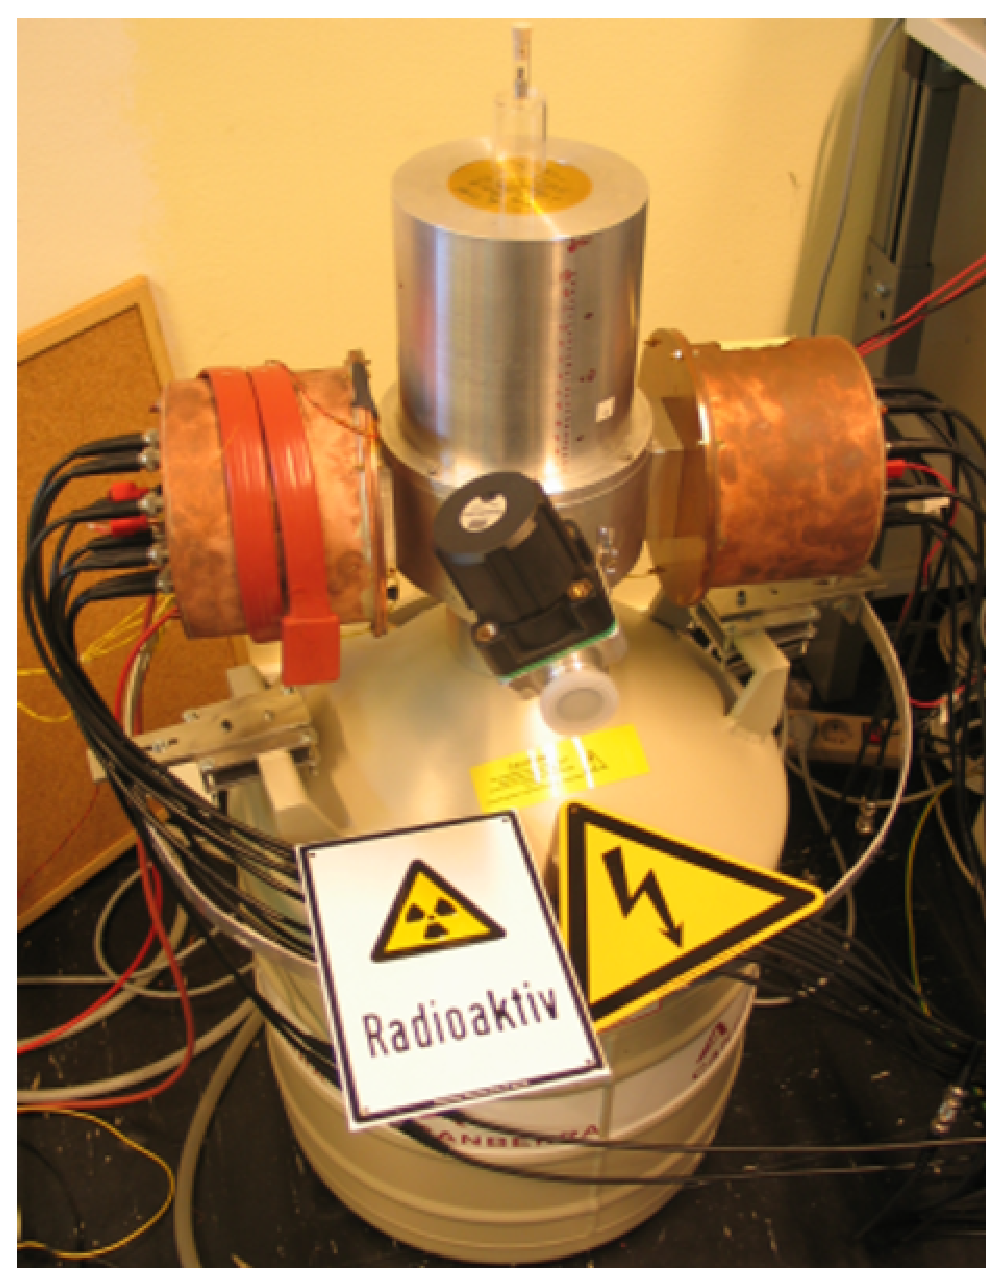
\includegraphics[height=0.25\textheight]{comcryo}}\hfil%
\subfloat[]{\label{fig:tt:ear}
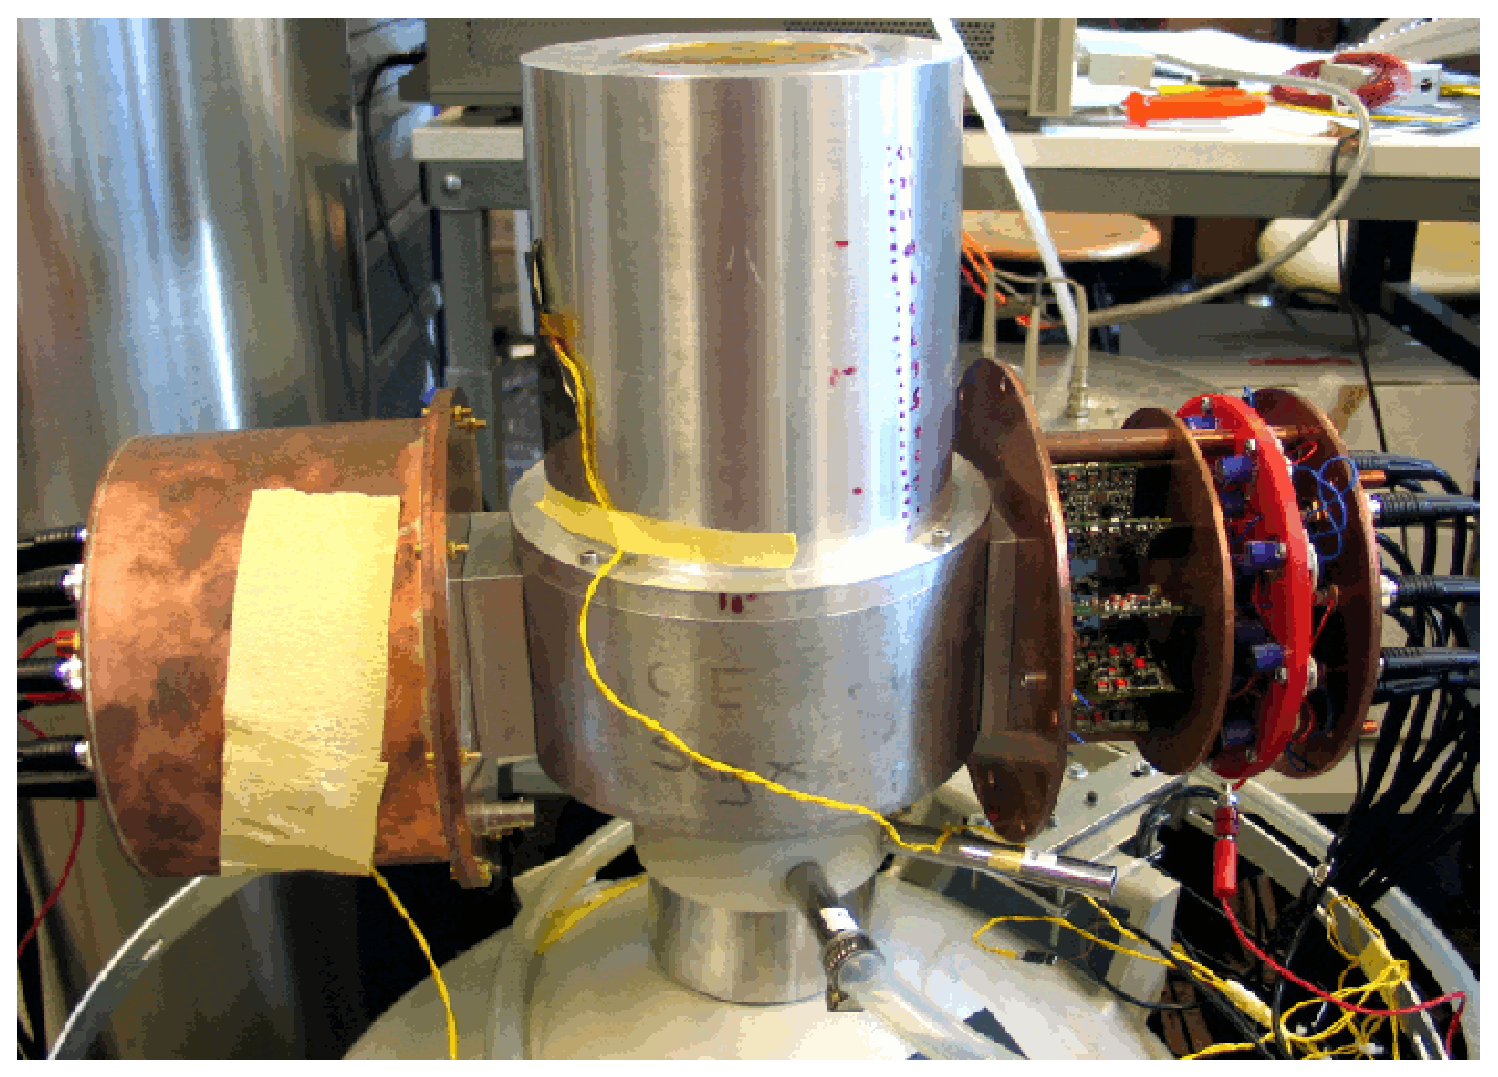
\includegraphics[height=0.25\textheight]{SIears}}%
\caption{Test cryostat developed by Canberra-France: (a) the standard
liquid nitrogen dewar with the vacuum can on top and (b) a close-up of
the vacuum can and the copper ``ears'' housing the pre-amplifier
boards.}
\label{fig:tt:comcryo}
\end{figure}

\subsection{Gerdalinchen II}
\label{sec:tt:gii}
Gerdalinchen II (GII) is a special cryostat developed by the technical
division of the Max-Planck-Institut f\"ur Physik to test the operation
of up to three segmented germanium detectors submerged in cryogenic
liquid. Figure~\ref{fig:tt:g2} is a schematic of the main body of GII,
a two-walled cryogenic dewar inside a cylindrical aluminum tank with a
height of 960~mm and a diameter of 612~mm. The top flange can be moved
up, allowing the mounting of detectors to a vertical stainless steel
bar attached to the bottom of the flange, see
Fig.~\ref{fig:tt:g2d}. Figure~\ref{fig:tt:g2n} shows GII in operation
with a neutron source placed on its side. For more details please see
Fig.~\ref{fig:ii:sch} in the next chapter.

\begin{figure}[tbhp]
\centering
\subfloat[]{\label{fig:tt:g2}
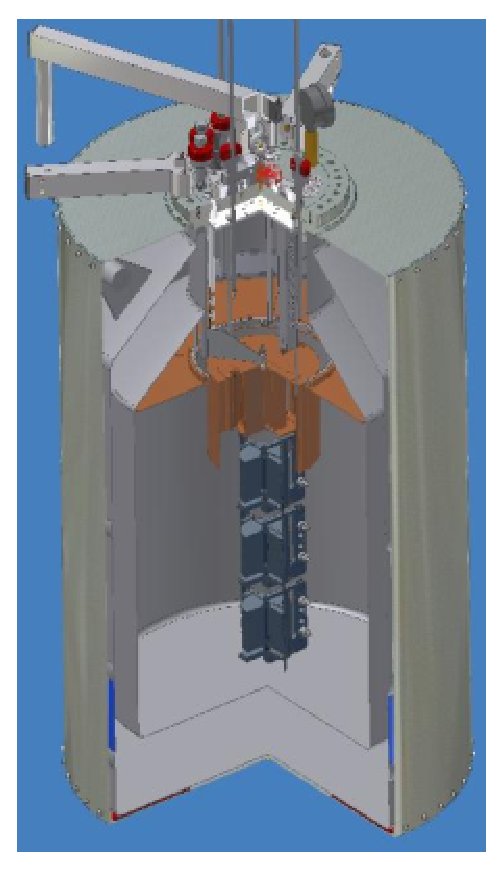
\includegraphics[height=0.25\textheight]{GIIdraw}}\hfil%
\subfloat[]{\label{fig:tt:g2n}
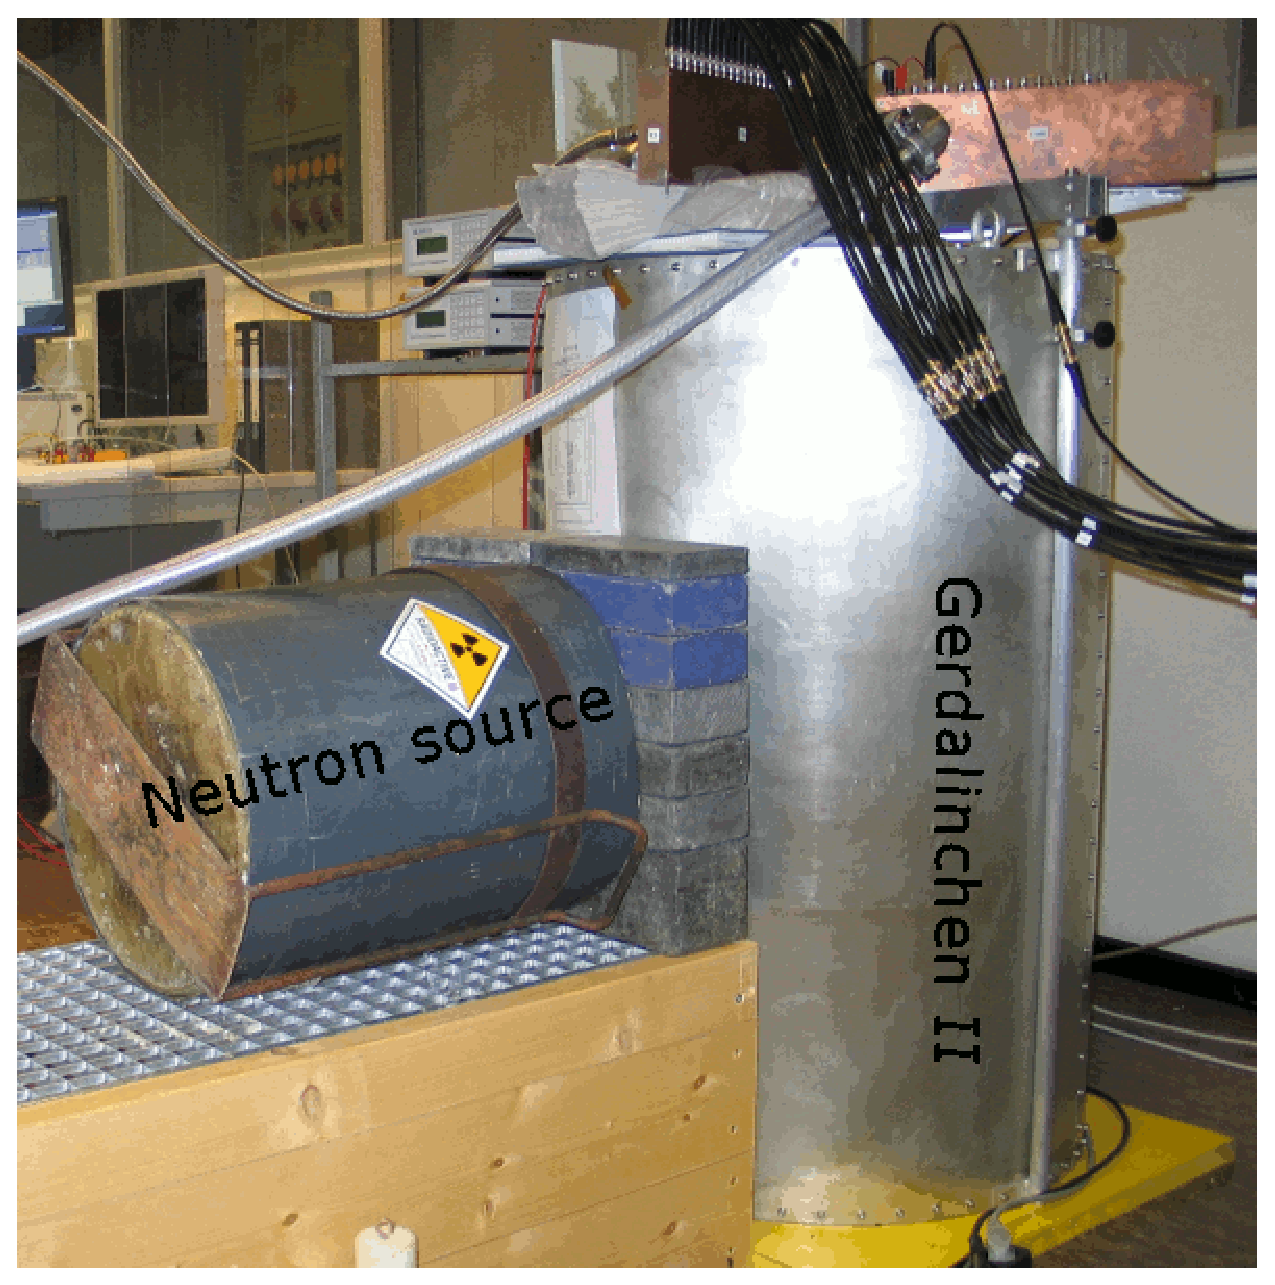
\includegraphics[height=0.25\textheight]{GIIneutron}}\hfil%
\subfloat[]{\label{fig:tt:g2d}
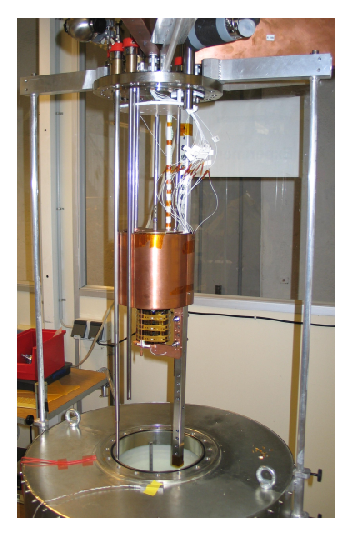
\includegraphics[height=0.25\textheight]{GIIdet}}%
\caption{Gerdalinchen II cryostat. (a) schematic of GII, (b) GII in
operation with a neutron source and (c) detector installation above
GII dewar.}
\label{fig:tt:gii}
\end{figure}

There are three high voltage feed-throughs and four signal connectors,
each with 18 channels, on the GII flange. This allows the operation of
up to three 18-fold segmented detectors simultaneously. The flange
also facilitates the re-filling of the dewar with cryogenic liquid and
the flushing with gaseous nitrogen without opening the system. The
dewar is re-filled daily to keep the level of the cryogenic liquid
above the infrared shields, and the liquid level is monitored using
several PT100 thermal resistances mounted at different places inside
the dewar (see Fig.~\ref{fig:ii:sch}).


\section{Electronics} 
\label{sec:tt:ele} 

\subsection{Front-end}
\label{sec:tt:fend} 
The read-out scheme of a segmented detector mounted inside the vacuum
cryostat is shown in Fig.~\ref{fig:tt:sifa}. The signals were read out
using charge sensitive PSC-823C pre-amplifiers with a decay time of
50~$\mu$s. The FET for the core electrode was mounted inside the
cryostat close to the detector, the FETs for the segment electrodes
were incorporated into the pre-amplifier boards which were housed
inside the copper ears on both sides of the detector as shown in
Fig.~\ref{fig:tt:ear}. Figure~\ref{fig:tt:sifb} depicts the layout of
the feed-throughs between the vacuum can and the copper ears.

\begin{figure}[tbhp]
\centering
\subfloat[]{\label{fig:tt:sifa}
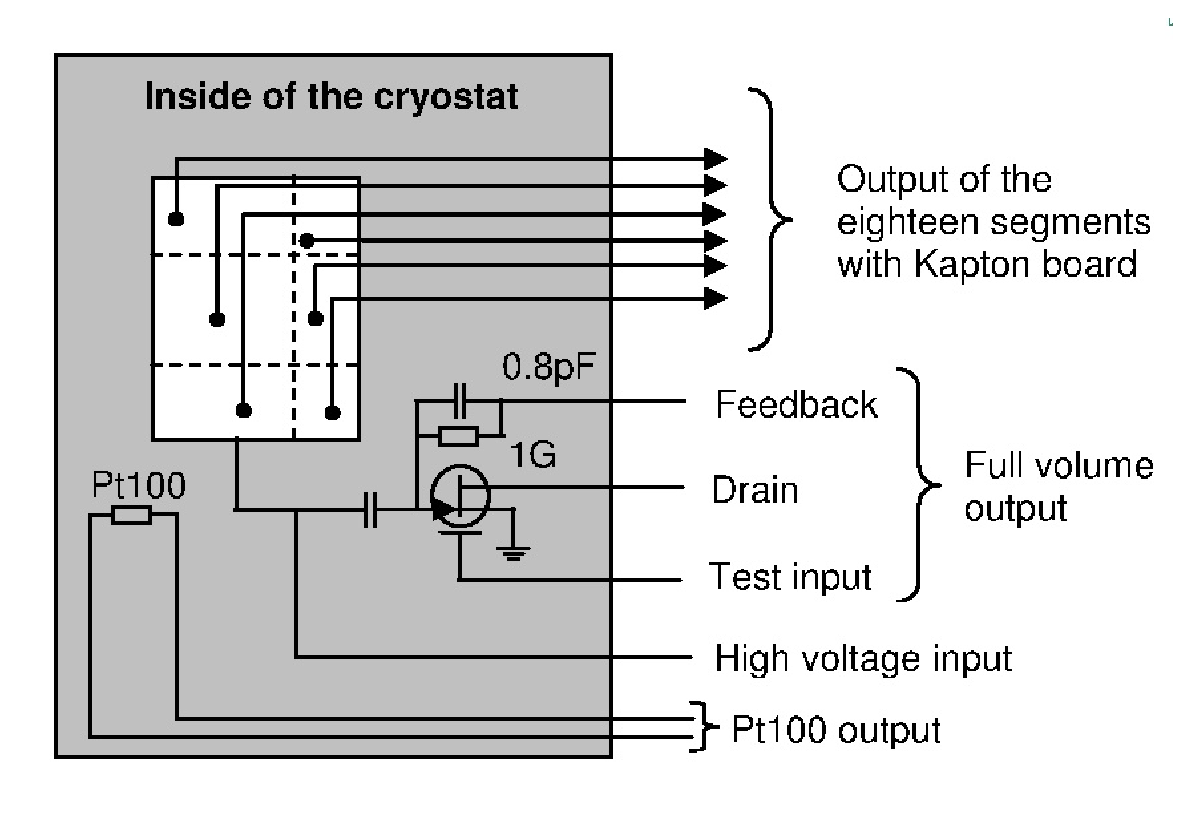
\includegraphics[height=0.25\textheight]{block1}}\hfil%
\subfloat[]{\label{fig:tt:sifb}
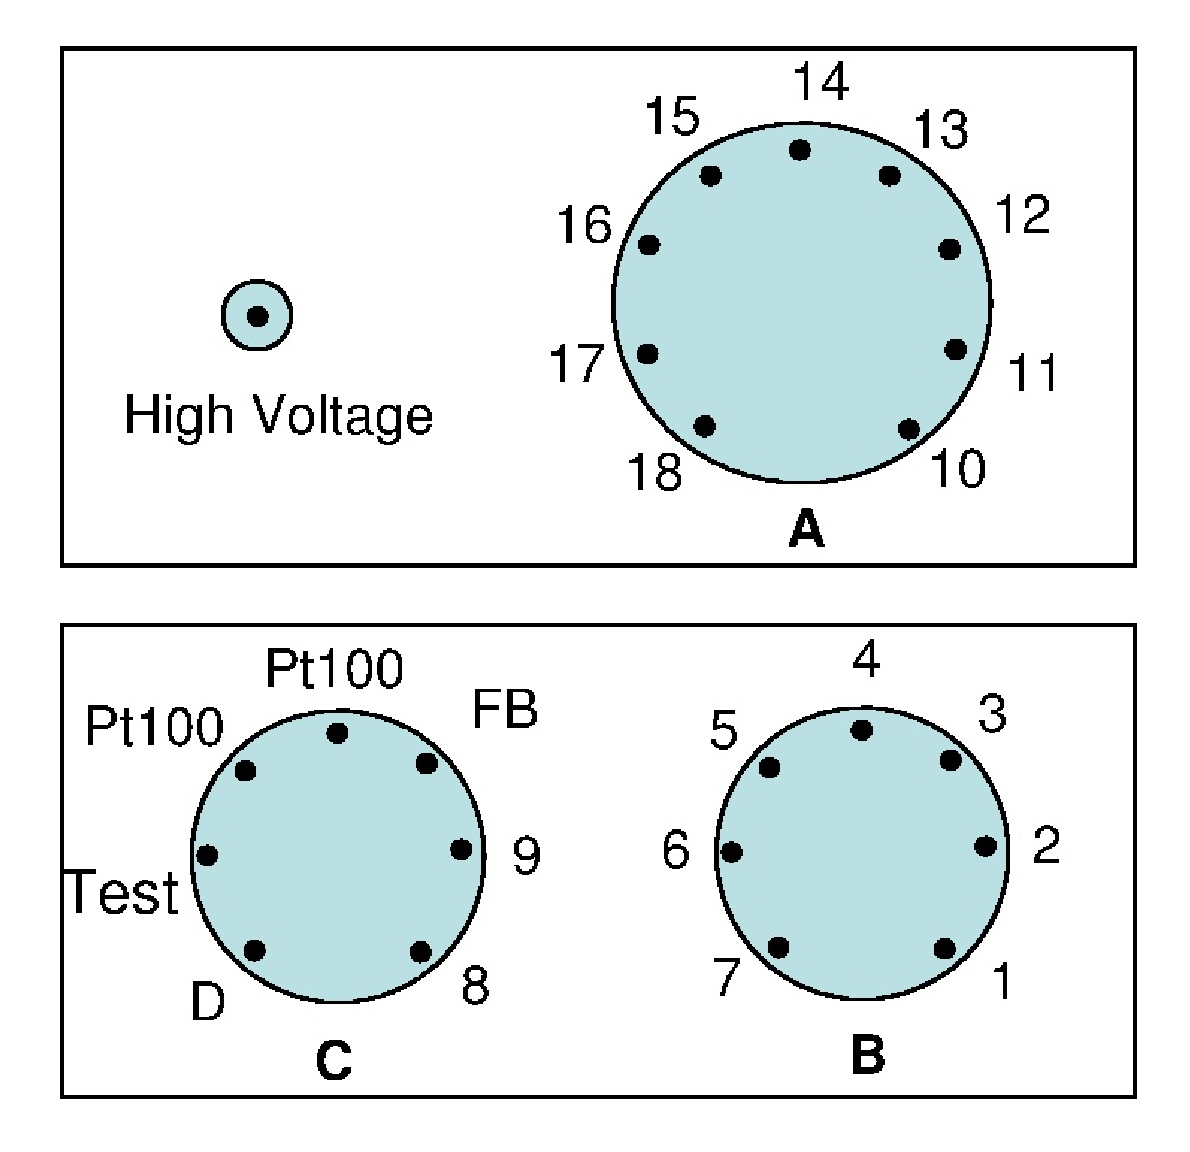
\includegraphics[height=0.25\textheight]{block2}}%
\caption{Frond-end electronics of a segmented detector mounted in the
vacuum cryostat: (a) read-out scheme and (b) layout of the
feed-throughs between the vacuum can and the copper ears.}
\label{fig:tt:sif}
\end{figure}

A different setup was used in GII. The FET for the core electrode was
incorporated into the pre-amplifier boards like for the segment
electrodes. Thus, the cross talk from the core signal to the segment
signals was minimized. All the pre-amplifier boards were mounted in a
copper box and shared a common ground as shown in
Fig.~\ref{fig:tt:gefb}. The filters for the high voltage lines and the
coupling capacitors for the core signal cables were placed under the
top flange as shown in Fig.~\ref{fig:tt:gefa}. They were first
operated above the cryogenic liquid level and later submerged for
better temperature stability.

\begin{figure}[tbhp]
\centering
\subfloat[]{\label{fig:tt:gefa}
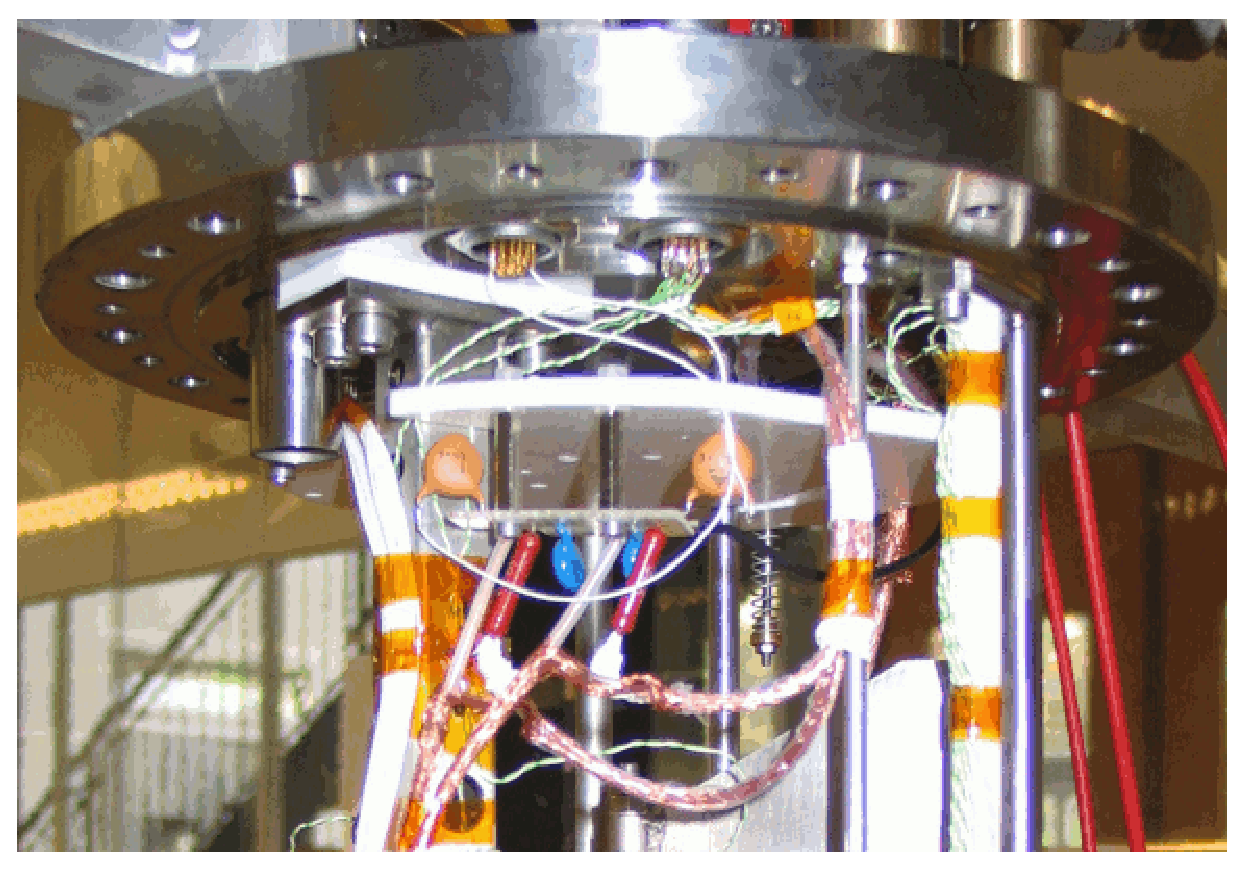
\includegraphics[height=0.2\textheight]{GIIHV}}\hfil%
\subfloat[]{\label{fig:tt:gefb}
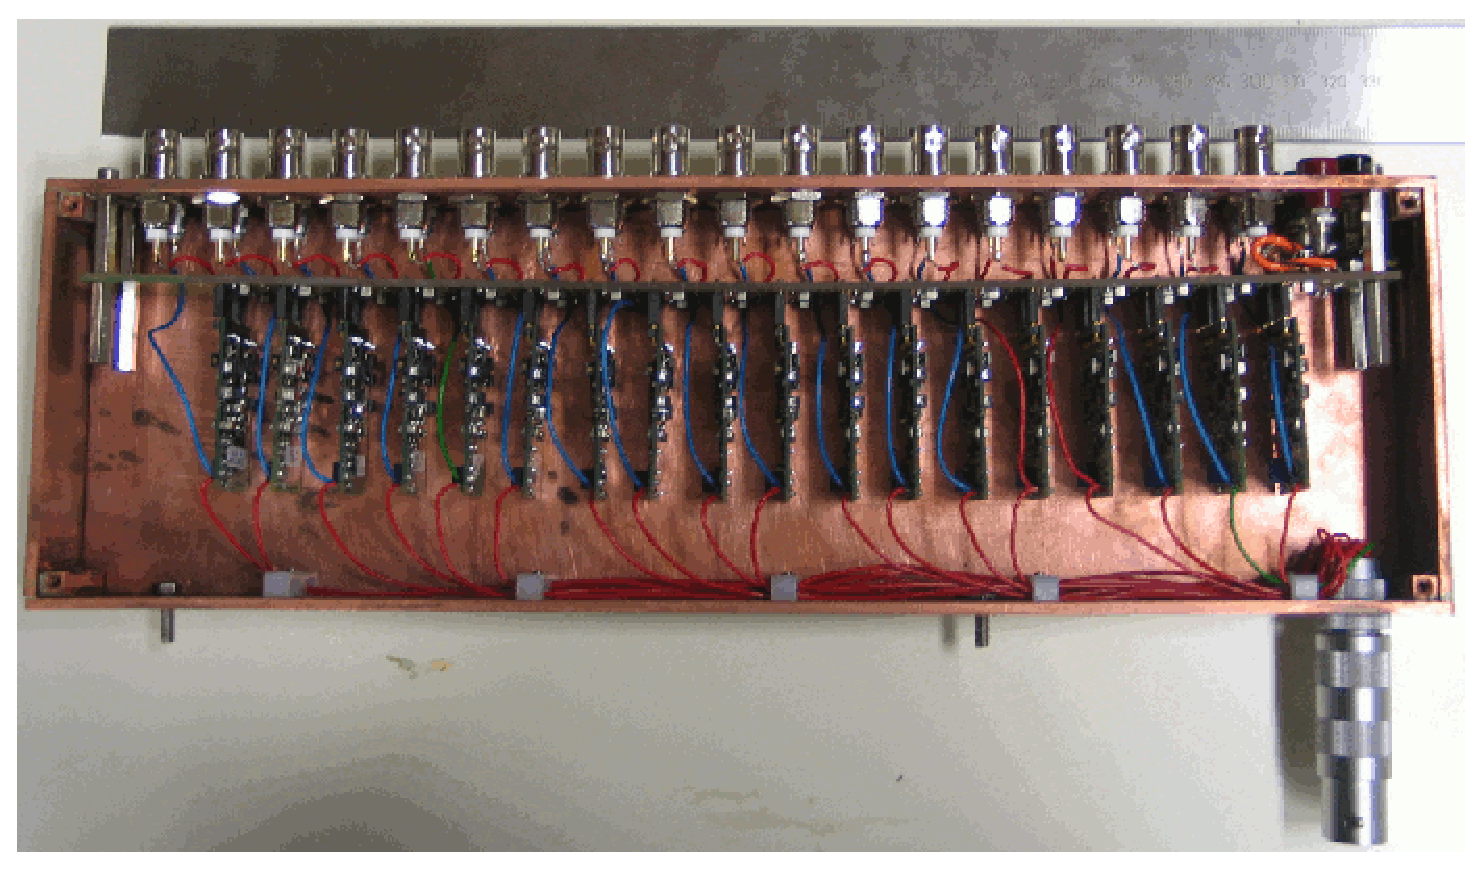
\includegraphics[height=0.2\textheight]{GIIpreamp}}%
\caption{Front-end electronics in GII: (a) high voltage filters and
coupling capacitors and (b) pre-amplifier box for a segmented
detector.}
\label{fig:tt:gef}
\end{figure}

\subsection{DAQ} 
\label{sec:tt:daq}
The pre-amplified signals are digitized using an XIA data acquisition
system \cite{Daq06} based on 14-bit ADC PIXIE-4 modules with a
sampling rate of 75~MHz. The bandwidth of the analog signals is
limited by a Nyquist filter to half the sampling rate, \textit{i.e.}
37.5~MHz. This avoids aliasing the noise from higher frequencies. It
is implemented in the analog section of the PIXIE-4 module as a
low-pass Sallen-Key filter resulting in a sharp cut-off at this
frequency. 

Energies of the pulses are calculated using software filters. In
principle, the energies of both positively and negatively polarized
pulses can be calculated. However, since the polarization of all
channels was set to be positive, there should not be any negative
pulse. The system was configured such that only the energies of
positive pulses were calculated and the energies of other kinds of
pulses were simply set to zero rather than calculated. This led to the
observation of a special type of events with negative pulses in some
of the channels as will be described in Chapter~\ref{cha:np}.

Recorded pulse shape data consist of 300 samples of the integrated
charge amplitude. The delay for the onset of the signal can be set by
hand and was set to 1~$\mu$s for most of the measurements. The trigger
and energy thresholds of the core and segment electrodes can be set to
different values. Pile-up pulses can be rejected or stored using a
rough energy estimation.


\section{Monitoring} 
\label{sec:tt:lamo}
The operation of the test facilities requires the monitoring of high
voltage supplies, temperature monitors, vacuum gauges, oxygen sensors,
etc.. The monitoring needs to be automated for overnight and long term
measurements. A generalized ``Laboratory Monitor system'', LaMo, was
developed to monitor and control most of the hardware in the
laboratories using the graphic programming language, LabVIEW. The
system has a set of user friendly interfaces to perform most of the
common lab tasks and a modularized design of the functionality to
facilitate the implementation of new pieces of hardware.

Figure~\ref{fig:tt:lamo} shows the most important control panels of
LaMo. The main panel is called ``Laboratory'' as shown in
Fig.~\ref{fig:tt:plab}. It shows a list of experiments going on in the
laboratory and their status. An experiment can be created, edited,
started, stopped using the buttons next to the experiment list. The
``Laboratory'' panel also provides functions common to all
experiments, such as email alerts, electricity, oxygen sensors,
etc.. Pieces of hardware to be associated to an experiment can be
chosen from a list of available hardware. This is done in the
``Config'' panel of LaMo as shown in Fig.~\ref{fig:tt:pcon}, where
pieces of hardware can be added or deleted from the list to be
monitored. Once an experiment is created and configured, it is started
from the ``Laboratory'' panel. An ``Experiment'' panel, as shown in
Fig.~\ref{fig:tt:pexp}, where monitored variables are shown in
different ways, automatically pops up. The functions specified for a
particular experiment can be executed from there.

\begin{figure}[tbhp]
\centering
\subfloat[]{\label{fig:tt:plab}
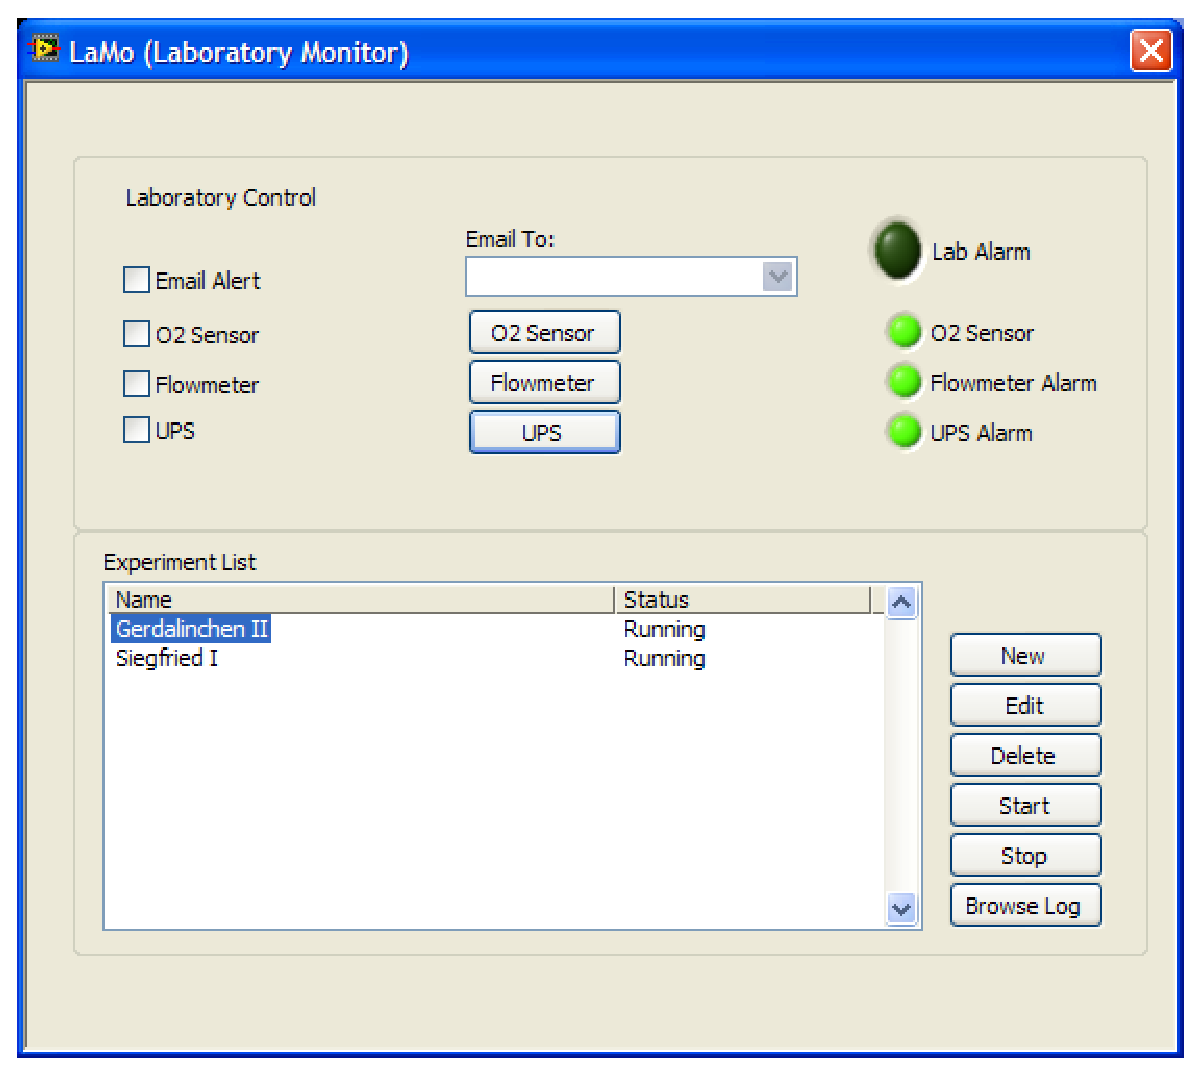
\includegraphics[height=0.23\textheight]{LaMoLab}}\hfil%
\subfloat[]{\label{fig:tt:pcon}
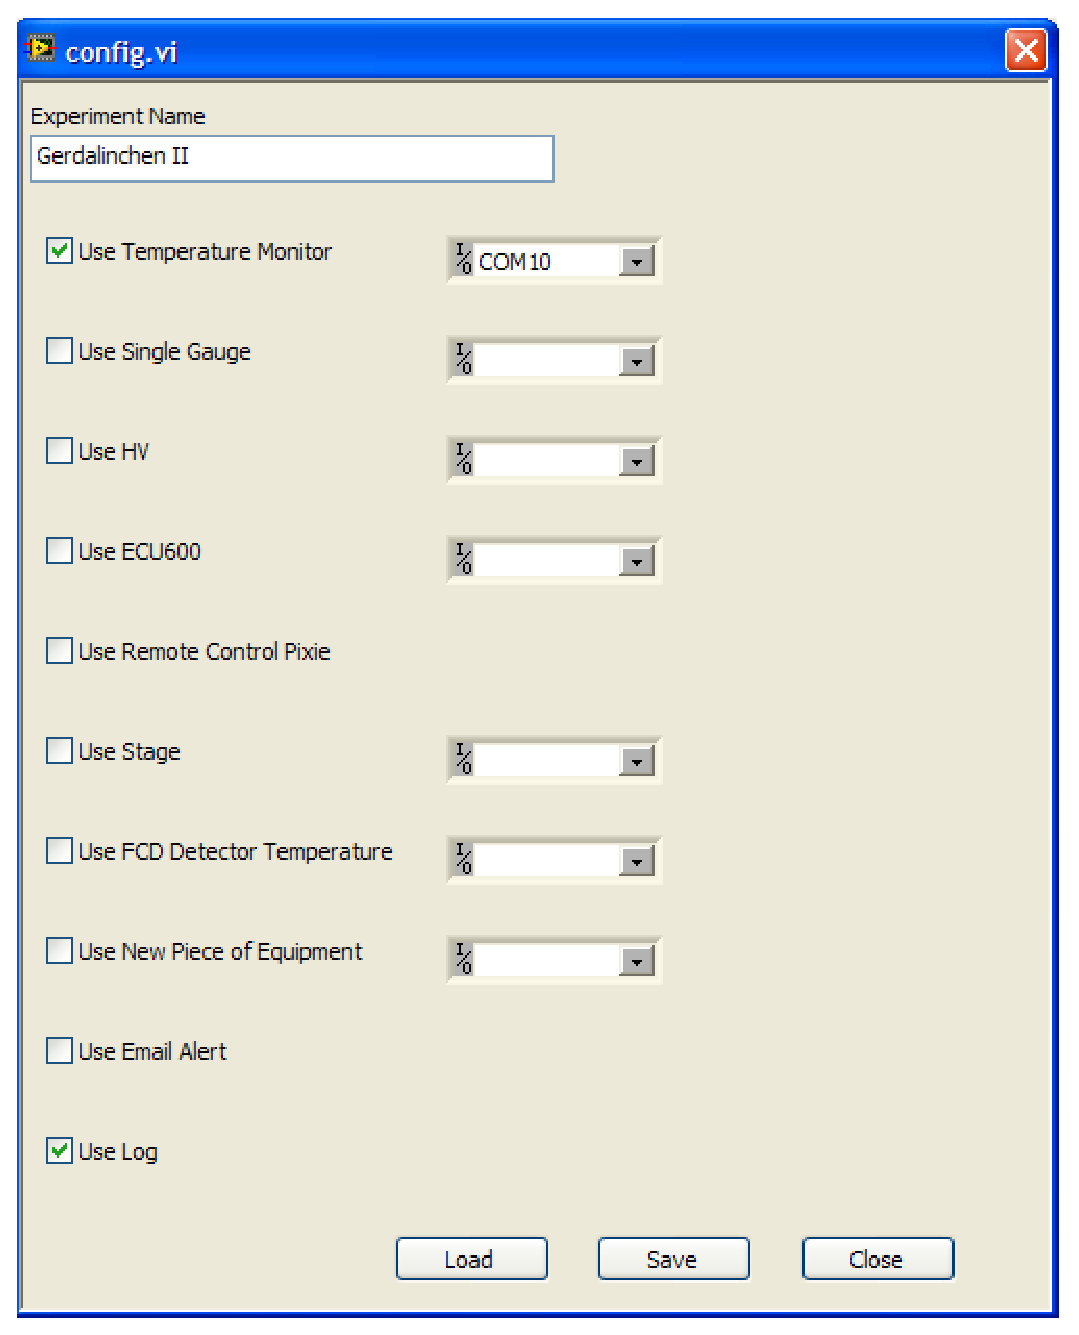
\includegraphics[height=0.23\textheight]{LaMoEdit}}\hfil%
\subfloat[]{\label{fig:tt:pexp}
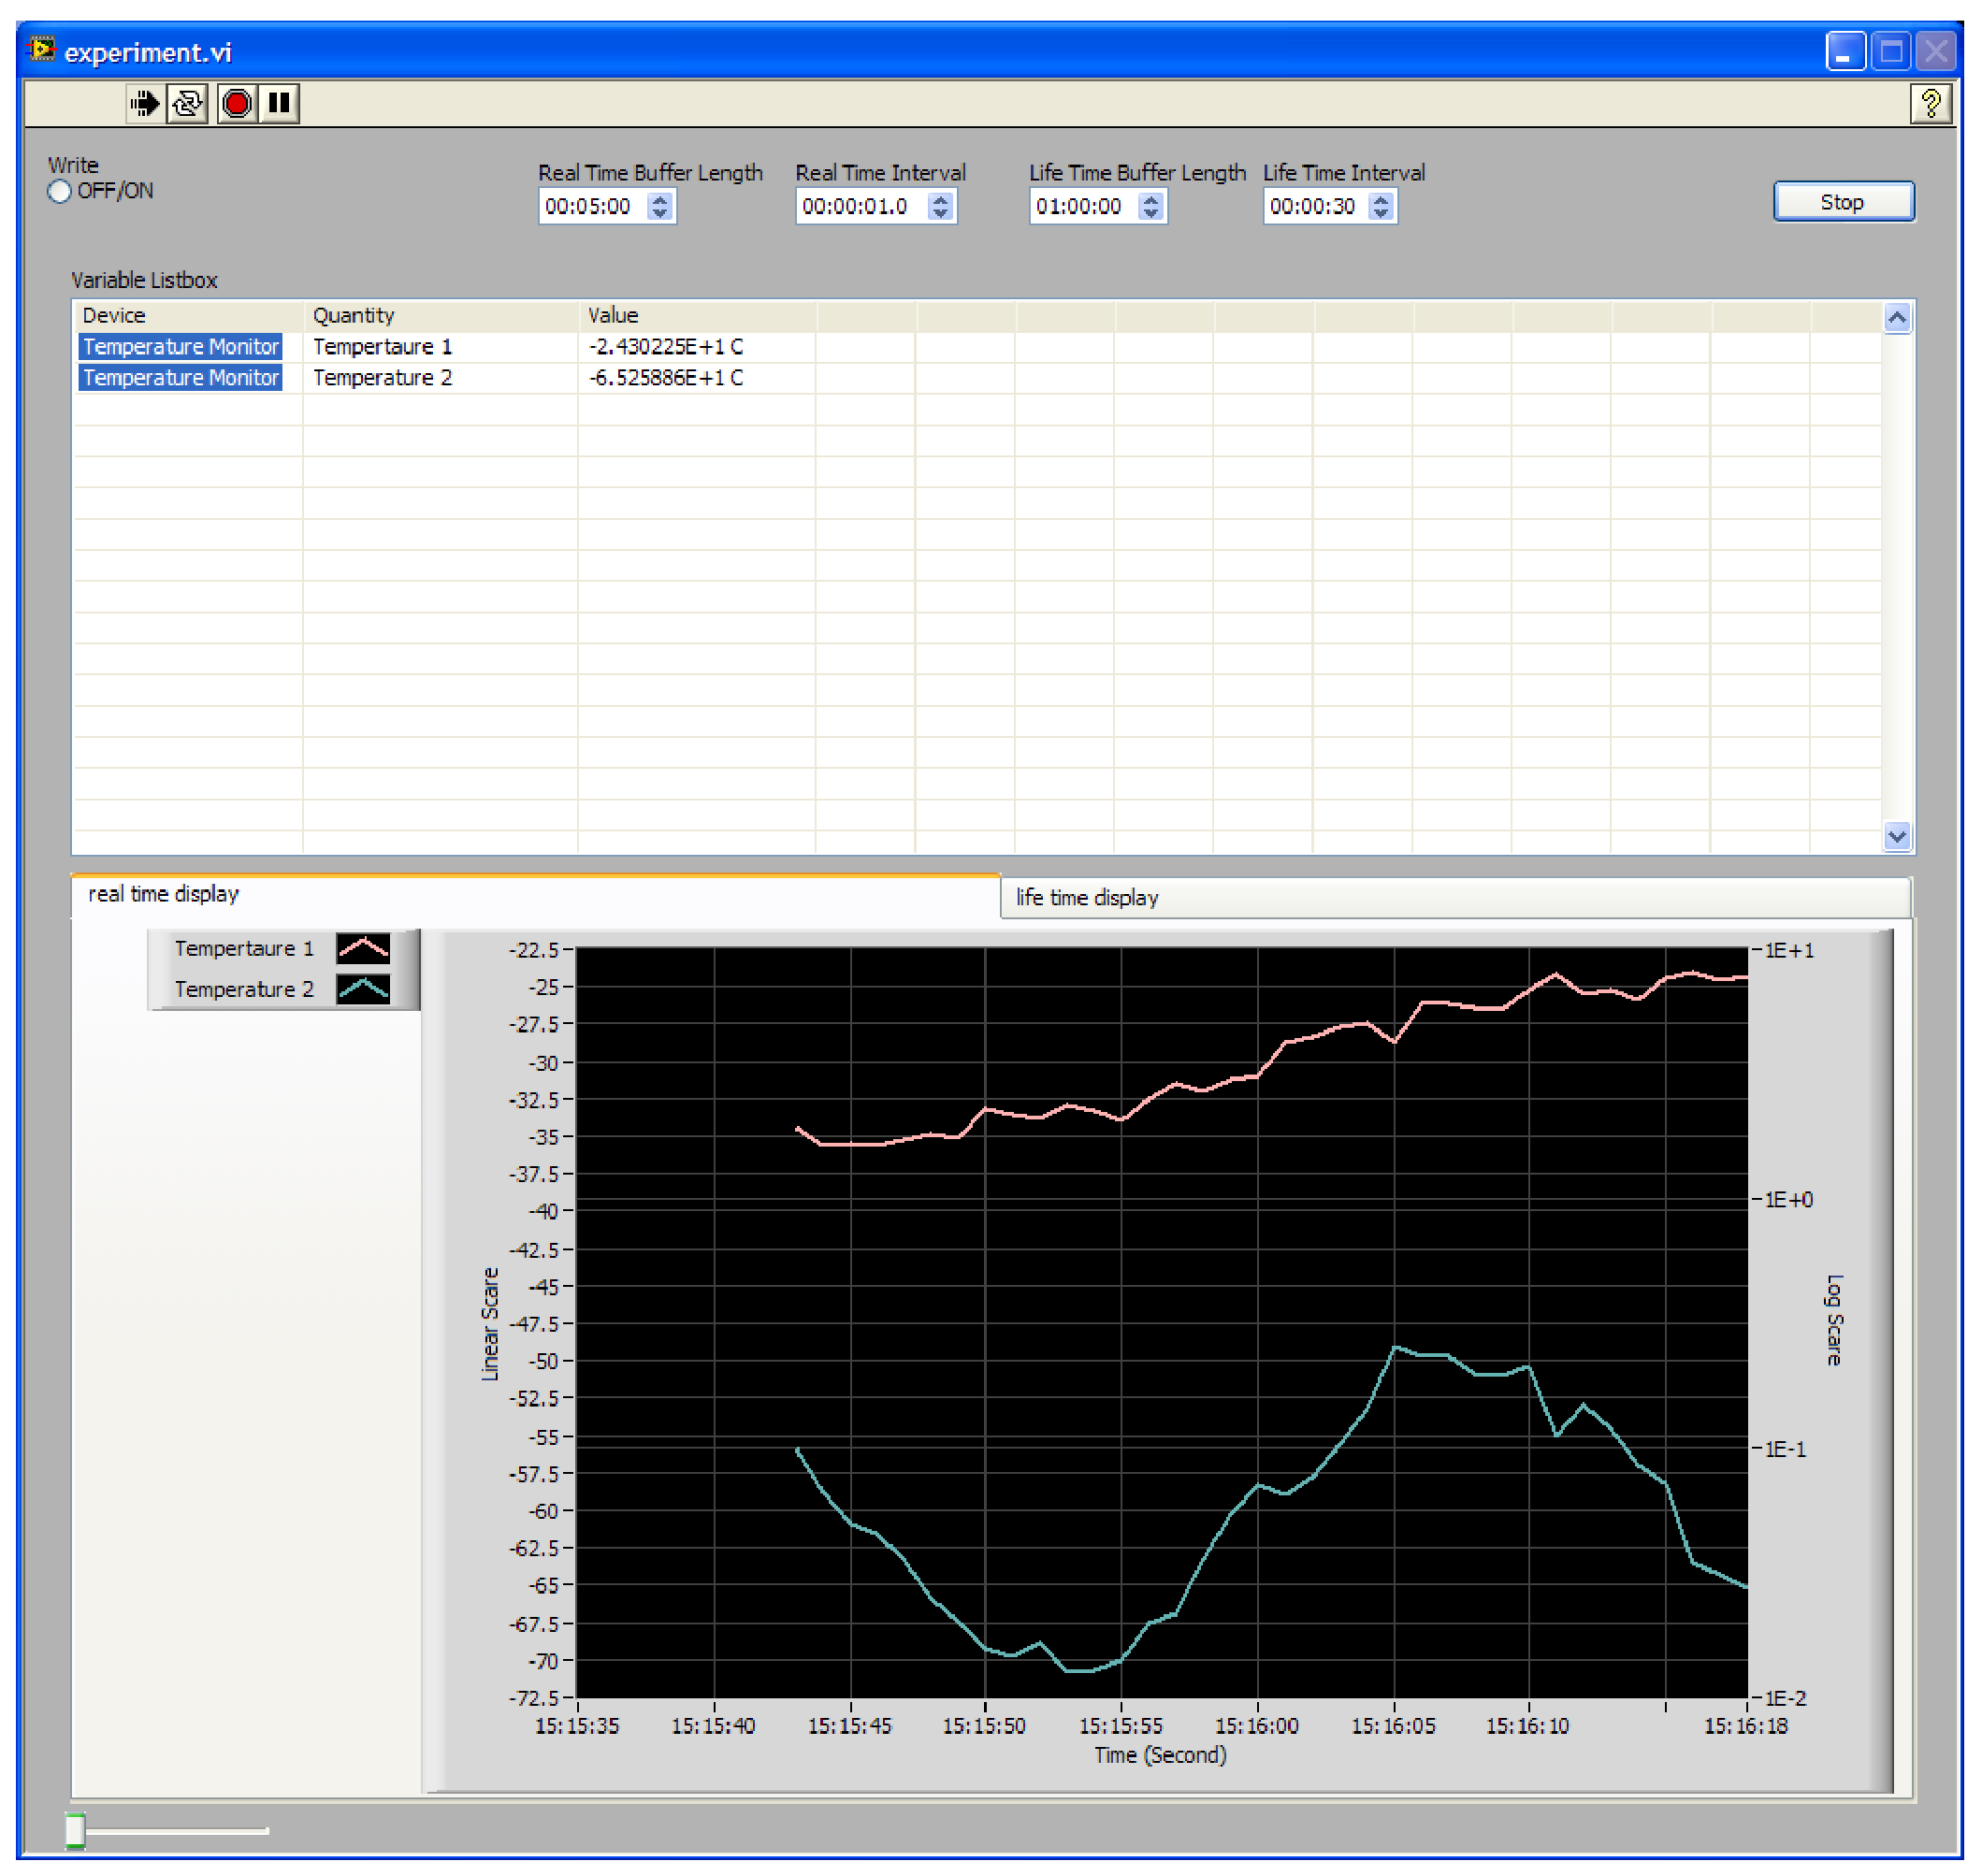
\includegraphics[height=0.23\textheight]{LaMoExp}}%
\caption{Main panels of LaMo: (a) ``Laboratory'' panel: it provides a
list of experiments and their status, and gives access to functions
common to all experiments; (b) ``Config'' panel: pieces of hardware to
be associated to an experiment can be added, deleted from the list to
be monitored; (c) ``Experiment'' panel: various displays of monitored
variables can be requested and the execution of experimental tasks can
be steered.}
\label{fig:tt:lamo}
\end{figure}

The common user interface enforces common I/Os for different pieces of
hardware. The functionality of LaMo is modularized so that the effort
to implement a new piece of hardware is minimized. To add a new piece
of equipment the developer only needs to define its I/O interface to
LaMo. The other efforts, such as programming the user interface, etc.,
do not have to be repeated every time.


%%% Local Variables:
%%% mode:latex
%%% TeX-master: "thesis"
%%% End:
